\vspace{-0.5cm}
\section*{Generell}
Die numerischen Datentypen sind gleichermaßen zu behandeln wie in den bekannten Programmiersprachen.

	\begin{minipage}[t]{12.5cm}
		\subsection*{Datentypen}
			\rowcolors{1}{blue!10}{white}
			\begin{tabular}{|>{\bfseries}l l l|}
				\hline Datentyp & \bfseries{Beschreibung} & \bfseries{False-Wert}
				\\\hline NoneType & Indikator für nichts & None
				\\\hline \multicolumn{3}{|l|}{\bfseries{Numerische Datentypen}}
				\\ int & Ganze Zahlen & 0
				\\ float & Gleitkommazahlen & 0.0
				\\ bool & Boolesche Werte & False
				\\ complex & Komplexe Zahlen & 0 + 0j
				\\\hline \multicolumn{3}{|l|}{\bfseries{Sequenzielle Datentypen}}
				\\ str & Zeichenketten oder Strings(unveränderlich) & ' '
				\\ list & Listen(veränderlich) & []
				\\ tuple & Tupel(unveränderlich) & ()
				\\ bytes & Sequenz von Bytes(unveränderlich) & b' '
				\\ bytesarray & Sequenz von Bytes(veränderlich) & bytearray(b' ')
				\\\hline Mengen & & 
				\\ set & Einmalig vorkommende Objekte & set()
				\\ frozenset & Wie set jedoch unveränderlich & frozenset()
				\\\hline \multicolumn{3}{|l|}{\bfseries{Assoziative Datentypen}}
				\\ dict & Dictionary(veränderlich) & { }
				\\\hline
			\end{tabular}
	\end{minipage}
		%\hspace*{1cm}
		\begin{minipage}[t]{3cm}
			%\vspace*{0.7cm}
			\subsection*{Operatoren}
				\rowcolors{1}{blue!10}{white}
				\begin{tabular}{|l l|}
					\hline \bfseries{Operator} & \bfseries{Beschreibung} \\\hline
					x // y & Ganzzahliger Quotient\\
					x ** y & Potenzieren, $x^y$ \\ 
					+,-,... & Übliche Operation\\\hline
				\end{tabular}
			\subsection*{Variablen}
				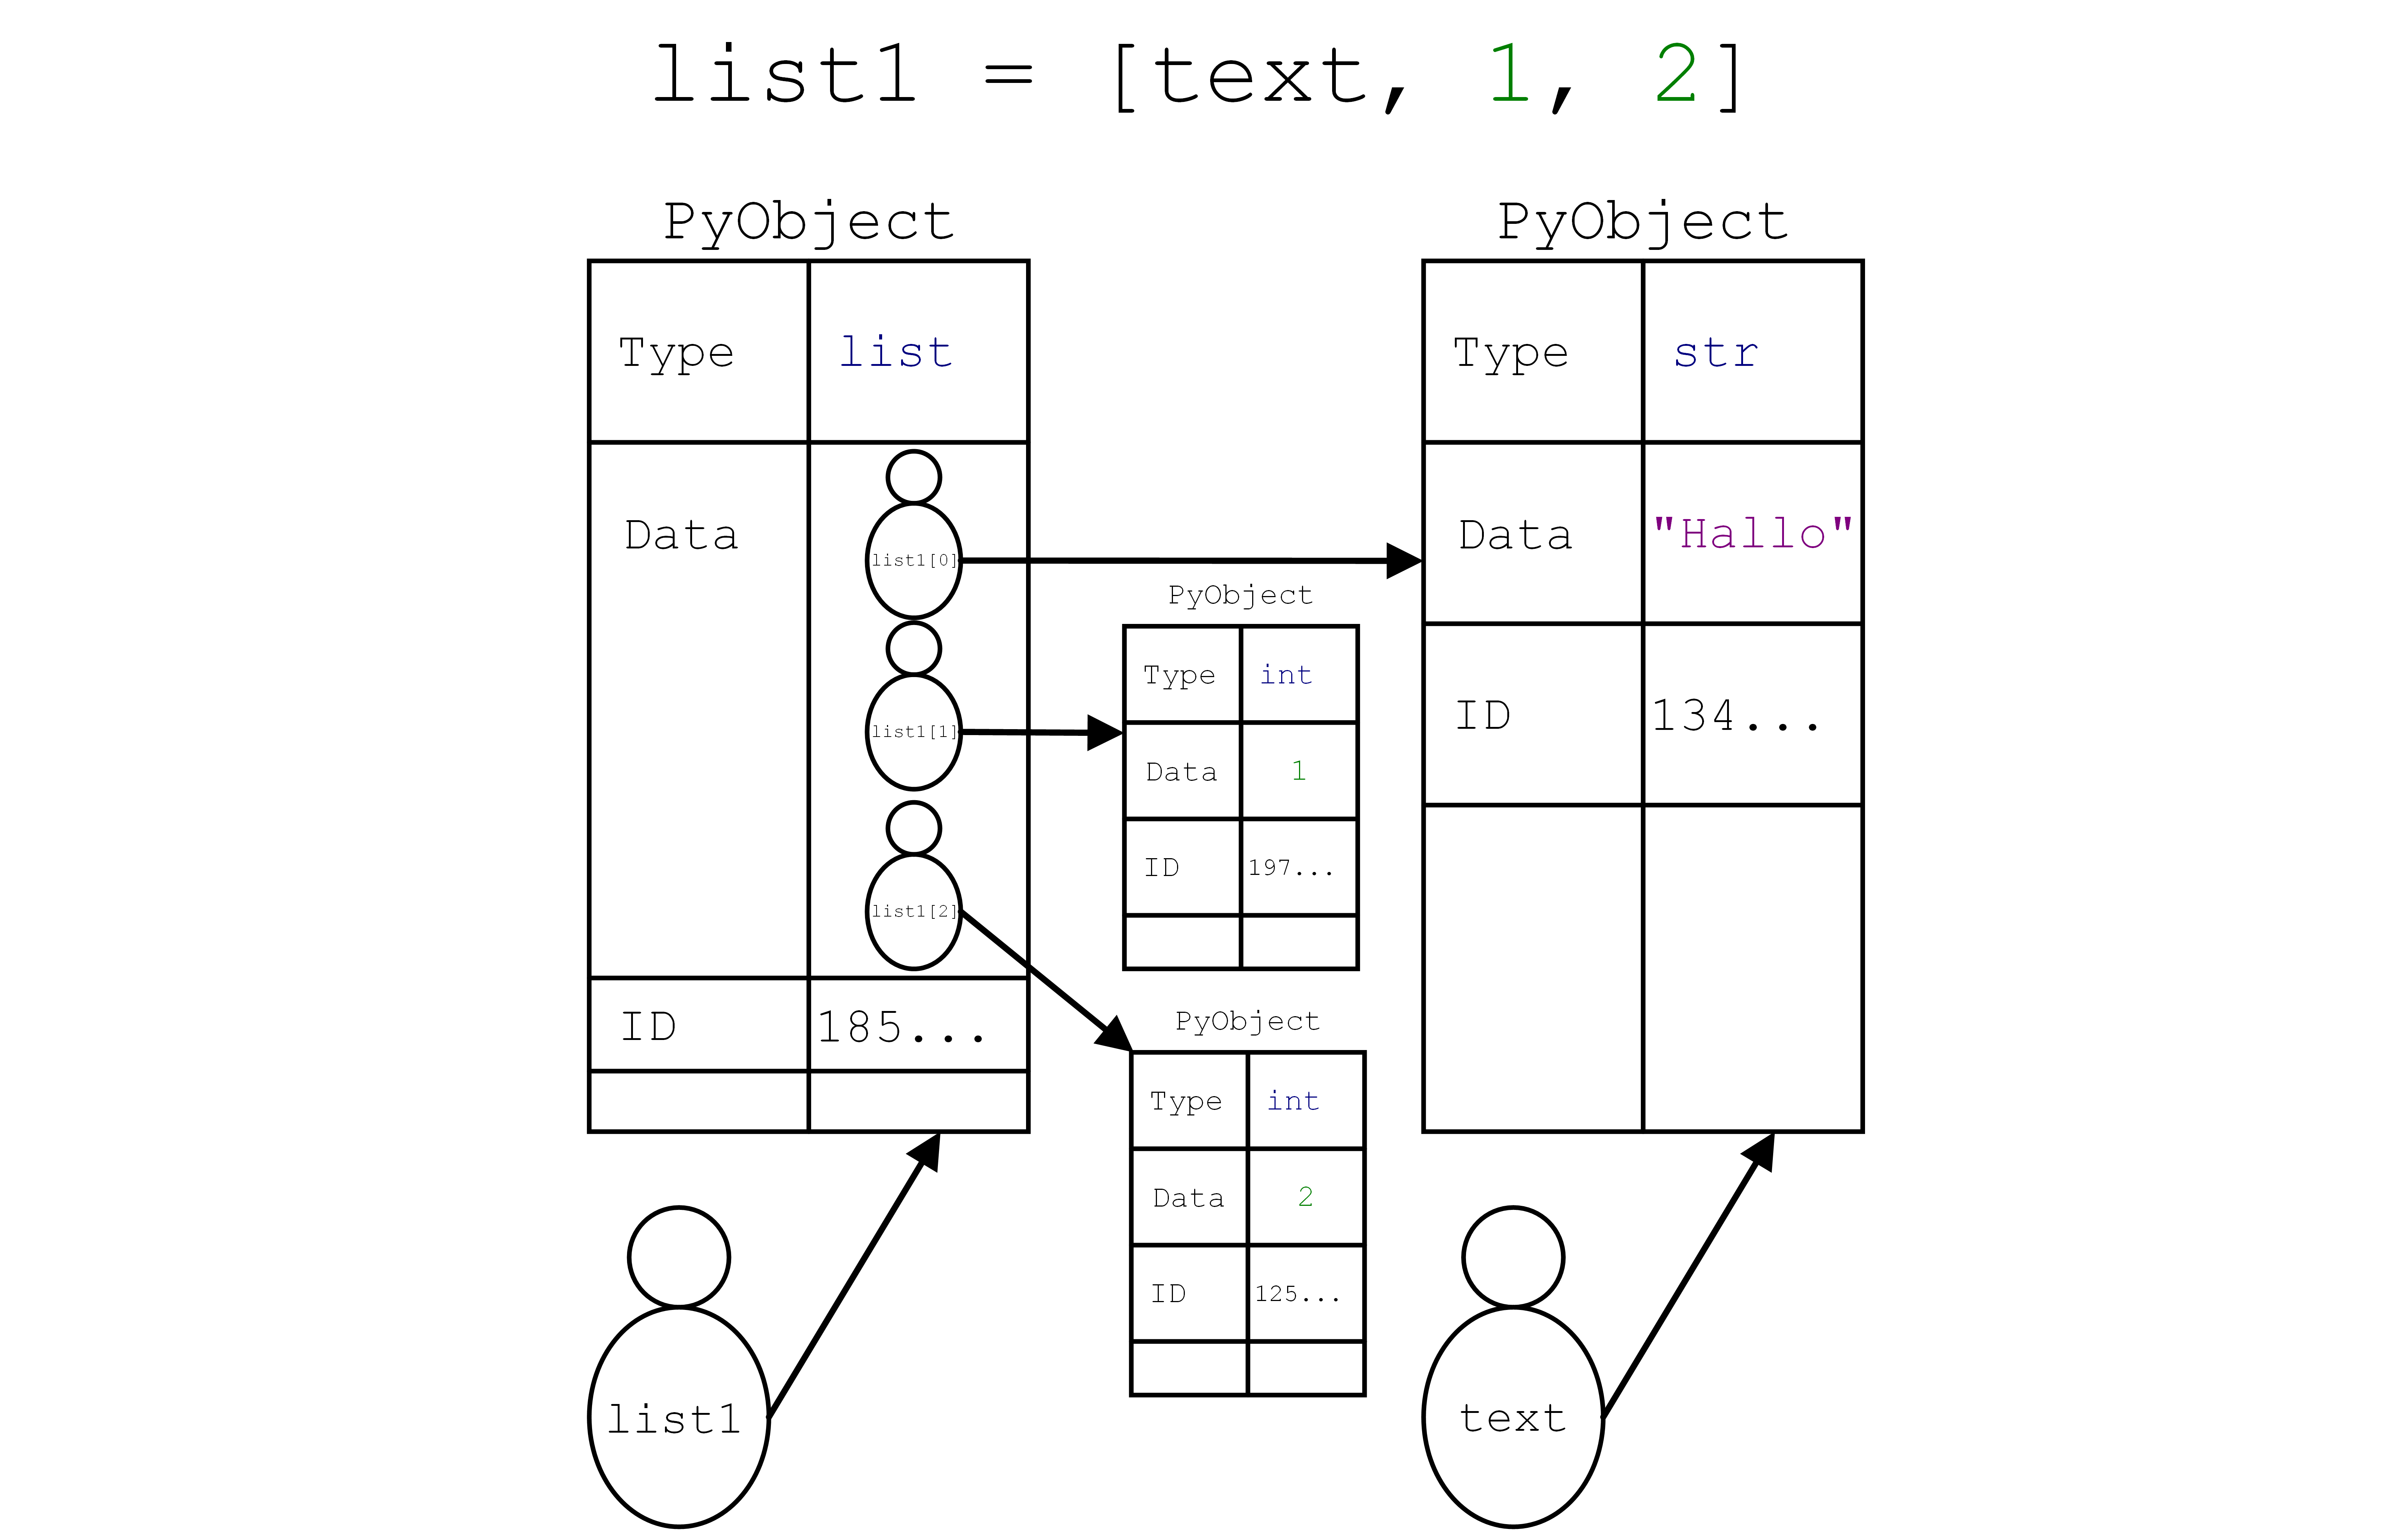
\includegraphics[height=4.5cm, align=t]{pics/Variablen.PNG}
		\end{minipage}
	\subsection*{Casting}
	\hspace{2cm}
	\rowcolors{1}{blue!10}{white}
	\begin{tabular}{|l l l | l l l|}
		\hline \bfseries{Datentyp} & \bfseries{Klasse} & \bfseries{Direkt} & \bfseries{Datentyp} & \bfseries{Klasse} & \bfseries{Direkt}
		\\\hline Ganzzahl & int() & 3 & Gleitkommazahl & float() & 3.1415
		\\ Boolescher Wert & bool() & True,False & Komplexe Zahl & complex() & 2 + 4j
		\\ String & str() & "HSR",'OST' & Liste & list() & [1,2,3]
		\\  Menge & set() & {1,2,3} & Tupel & tuple() & (1,2,3)
		\\ Unver. Menge & frozenset() & frozenset({1,2,3}) & Dictionary & dict() & {}, {"Key": 1}
		\\\hline
	\end{tabular}
	\subsection*{Eingabe und Ausgabe}
		\begin{minipage}[h]{7cm}
			\lstinputlisting{code/Streams.py}
			\textcolor{red}{\textbf{In:}}
			\\type your name:MFG GG OG
			\\\textcolor{red}{\textbf{Out:}}
			\\Hello MFG GG OG
			\\YES--WE--CAN--
		\end{minipage}
		\begin{minipage}[t]{8cm}
		\rowcolors{1}{blue!10}{white}
			\begin{tabular}{|l l l|}
				\hline \bfseries{Parameter} & \bfseries{Beschreibung} & \bfseries{Default}
				\\\hline object(s) & Alle Objekte werden in String konvertiert & 
				\\ sep='seperator' & Separierung der Objekte & ' '
				\\ end='end' & Letztes Zeichen des print-Befehl & '\textbackslash n'
				\\ file & Objekt mit einer Write-Methode & sys.stdout
				\\ flush & Boolscher Wert für die Output-Überprüfung & False
				\\\hline
			\end{tabular}
		\end{minipage}